%%%%%%%%%%%%%%%%%%%%%%%%%%%%%%%%%%%%%%%%%
% Dreuw & Deselaer's Poster
% LaTeX Template
% Version 1.0 (11/04/13)
%
% Created by:
% Philippe Dreuw and Thomas Deselaers
% http://www-i6.informatik.rwth-aachen.de/~dreuw/latexbeamerposter.php
%
% This template has been downloaded from:
% http://www.LaTeXTemplates.com
%
% License:
% CC BY-NC-SA 3.0 (http://creativecommons.org/licenses/by-nc-sa/3.0/)
%
%%%%%%%%%%%%%%%%%%%%%%%%%%%%%%%%%%%%%%%%%

%----------------------------------------------------------------------------------------
%	PACKAGES AND OTHER DOCUMENT CONFIGURATIONS
%----------------------------------------------------------------------------------------

\documentclass[final,hyperref={pdfpagelabels=false}]{beamer}

\usepackage[orientation=portrait,size=a0,scale=1.4]{beamerposter} % Use the beamerposter package for laying out the poster with a portrait orientation and an a0 paper size

\usetheme{I6pd2} % Use the I6pd2 theme supplied with this template

\usepackage[english]{babel} % English language/hyphenation

\usepackage{amsmath,amsthm,amssymb,latexsym} % For including math equations, theorems, symbols, etc

%\usepackage{times}\usefonttheme{professionalfonts}  % Uncomment to use Times as the main font
%\usefonttheme[onlymath]{serif} % Uncomment to use a Serif font within math environments

\boldmath % Use bold for everything within the math environment

\usepackage{booktabs} % Top and bottom rules for tables
\usepackage{amsmath}

\graphicspath{{figures/}} % Location of the graphics files

\usecaptiontemplate{\small\structure{\insertcaptionname~\insertcaptionnumber: }\insertcaption} % A fix for figure numbering

%----------------------------------------------------------------------------------------
%	TITLE SECTION 
%----------------------------------------------------------------------------------------

\title{\huge Simply use the force \\ \LARGE Implementation of RF-based gesture interaction} % Poster title

\author{Christoph Rauterberg, Mathias Velten, Stephan Sigg, Xiaoming Fu} % Author(s)

\institute{University of G\"ottingen} % Institution(s)

%----------------------------------------------------------------------------------------
%	FOOTER TEXT
%----------------------------------------------------------------------------------------

\newcommand{\leftfoot}{Christoph Rauterberg} % Left footer text

\newcommand{\rightfoot}{c.rauterberg@stud.uni-goettingen.de} % Right footer text

%----------------------------------------------------------------------------------------

\begin{document}
\large
\setlength{\parindent}{0cm}

\addtobeamertemplate{block end}{}{\vspace*{2ex}} % White space under blocks

\begin{frame}[t] % The whole poster is enclosed in one beamer frame

\begin{columns}[t] % The whole poster consists of two major columns, each of which can be subdivided further with another \begin{columns} block - the [t] argument aligns each column's content to the top

\begin{column}{.02\textwidth}\end{column} % Empty spacer column

\begin{column}{.465\textwidth} % The first column

%----------------------------------------------------------------------------------------
%	OBJECTIVES
%----------------------------------------------------------------------------------------

% \begin{block}{Objectives}
% 
% \begin{enumerate}
%  \item Evaluate online learning of gestures (?)
%  \item Propose Showcase Application that highlights the use of online-learned gestures
% \end{enumerate}
% 
% 
% \end{block}

%----------------------------------------------------------------------------------------
%	MATERIALS
%----------------------------------------------------------------------------------------

\begin{block}{Motivation}
Recent approaches were able to achieve gesture interaction using \emph{specialised hardware}. We were aiming for \emph{online detection of gestures} based in the RF-signal strength.

\end{block}

\begin{block}{Related Work}
Sigg et al. observed that 10 RSSI packets per second are sufficient
to distinguish between simple classes and also hand gestures
in proximity of the receiver
\end{block}

%----------------------------------------------------------------------------------------
%	METHODS
%----------------------------------------------------------------------------------------
\begin{block}{A showcase application}
We developed two showcase applications, where the user is able to \emph{train} certain gestures in a given scenario and is then able to \emph{control a slideshow} with these gestures or \emph{take a snapshot} with the camera of the mobile phone when a certain gesture is detected.
\begin{figure}
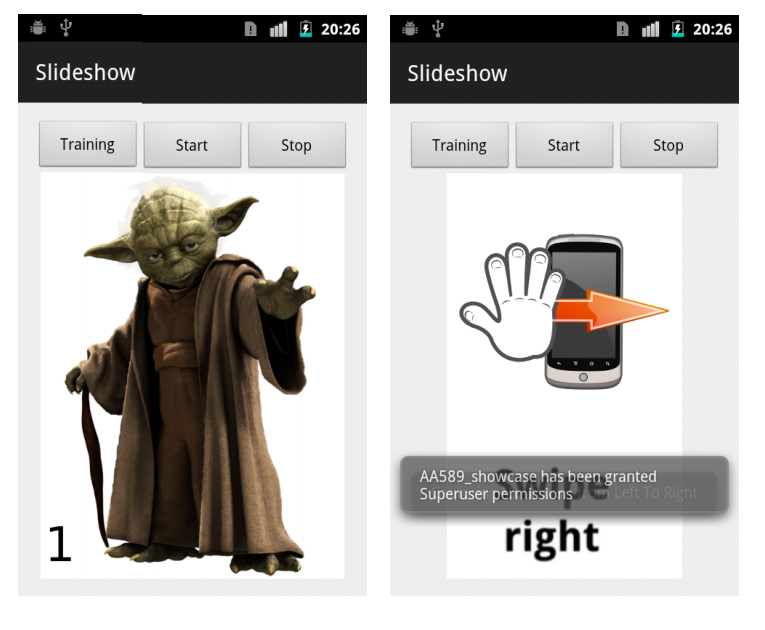
\includegraphics[width=0.9\linewidth]{./pics/showcaseApp.png}
\caption{The UI of the showcase application. The user can swipe over the phone to display the next picture in the slideshow}
\label{fig:ushahidi}
\end{figure}
\end{block}



\begin{block}{Technical Details}
In order to improve recognition rates compared to previous work in the literature, we employ further features from the data:
\begin{enumerate}
\item The user will be asked to perform movements for a period of time $t$. 
This data will be recorded and stored into a file.
\item The recorded data will be divided into $n$ slots. 
Each packet is sorted into a slot according to its \emph{time stamp}.
\item We then use statistical analysis to compute the \emph{features} for Machine Learning. 
Those features are for one timeslot the \emph{statistical mean}, \emph{standard derivation}, \emph{highest} recorded RSSI value and \emph{lowest} recorded RSSI value, \emph{total number} of packets as well as \emph{numerical representation} of the source MAC-Addresses.

\item With these features, we use a \emph{k-nearest-neighbour}-Classifier to classify the data.
\end{enumerate}


\end{block}

%----------------------------------------------------------------------------------------
%	MATHEMATICAL SECTION
%----------------------------------------------------------------------------------------




%----------------------------------------------------------------------------------------

\end{column} % End of the first column

\begin{column}{.03\textwidth}\end{column} % Empty spacer column
 
\begin{column}{.465\textwidth} % The second column



\begin{block}{Gesture Control}
We used the following clases within the slide show:
\begin{figure}

\centering
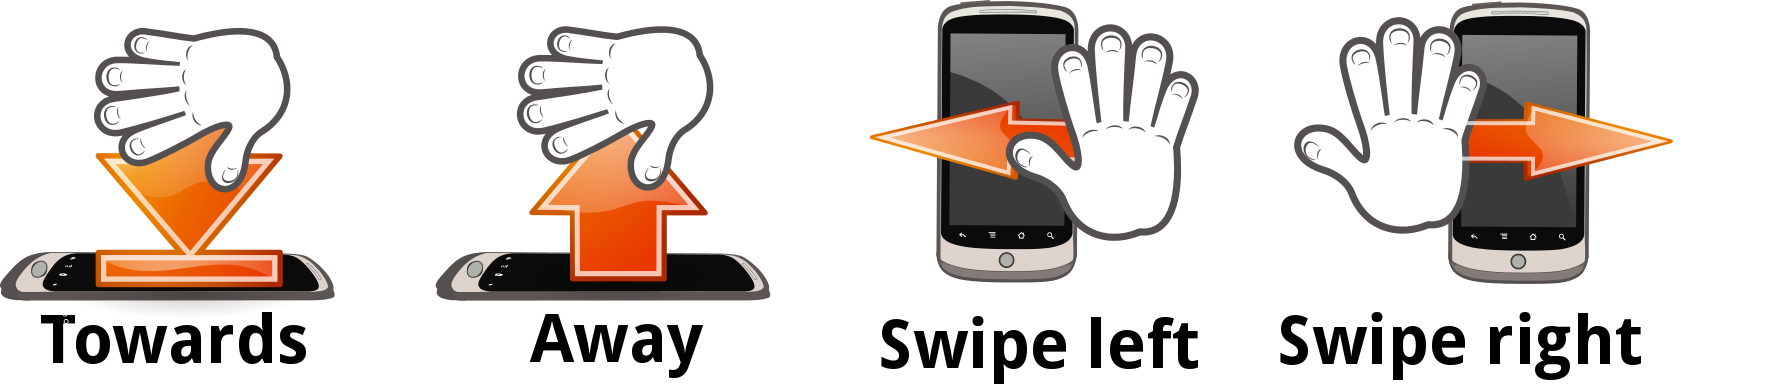
\includegraphics[width=.9\columnwidth]{./pics/gestures3}
\caption{All gestures considered. The Showcase Slideshow uses swipes over the phone to navigate within the slideshow.}
\label{fig:classes}
\end{figure}

\end{block}

%----------------------------------------------------------------------------------------
%	SOLUTION
%----------------------------------------------------------------------------------------

\begin{block}{Evaluation}
To evaluate the performance of the proposed method we evaluate the performance in the following scenarios:
\begin{description}
\item[Standard: ] After a training phase, while holding the phone in the hand, we record test samples to evaluate the accuracy of the classification. 
We will refer to this scenario as the \emph{standard scenario}.
\item[Training: ] We train the classifier whilst holding the phone \emph{on a certain spot in a certain room} and then \emph{walk about the room} and evaluate the classifier on different positions in the room.
\item[Ad-hoc:  ] We train the classifier whilst holding the phone \emph{on a certain spot in a certain room} and then \emph{completely leave the context} and go to other spaces within the city and evaluate the performance there. 
\end{description}


\begin{figure}
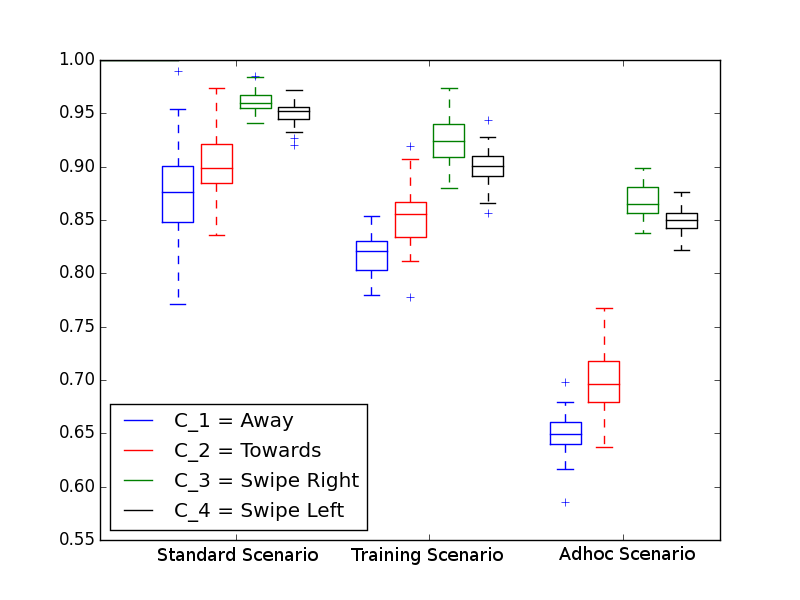
\includegraphics[width=0.9\linewidth]{./pics/boxcompare}
\caption{The results of the evaluation in the described scenarios.}
\end{figure}

\end{block}

%----------------------------------------------------------------------------------------
%	CONCLUSION
%----------------------------------------------------------------------------------------

\begin{block}{Conclusion}

\begin{enumerate}
 \item \large We are able to detect the used gestures with an accuracy of more than \emph{$90 \%$}.
 \item The proposed method is not robust to \emph{changes in the location}.
 \item The test, that have been described above, where all contucted in an environment with \emph{more than 10 packets per second}, as described by Sigg et al.
\end{enumerate}


\end{block}

% \begin{block}{References}
% \begin{enumerate}
%  \item Sigg et al.: Passive, device-free recognition on your mobile phone: tools, features and a case study 
%  \item 
% \end{enumerate}
% \end{block}

% \nocite{*} % Insert publications even if they are not cited in the poster
% \small{\bibliographystyle{unsrt}
% \bibliography{./pcan.bib}}
% \end{block}

%----------------------------------------------------------------------------------------
%	REFERENCES
%----------------------------------------------------------------------------------------

% \begin{block}{References}
%         
% \nocite{*} % Insert publications even if they are not cited in the poster
% \small{\bibliographystyle{plain}
% \bibliography{./pcan.bib}}
% 
% \end{block}

%----------------------------------------------------------------------------------------
%	ACKNOWLEDGEMENTS
%----------------------------------------------------------------------------------------

% \begin{block}{Acknowledgment}
% \small
% This research was funded by the joint EU FP7/NICT
% GreenICN Project, Contract No. 608518 and NICT No. 167.
% \end{block}

%----------------------------------------------------------------------------------------
%	CONTACT INFORMATION
%----------------------------------------------------------------------------------------

\setbeamercolor{block title}{fg=black,bg=orange!70} % Change the block title color

%----------------------------------------------------------------------------------------

\end{column} % End of the second column

\begin{column}{.015\textwidth}\end{column} % Empty spacer column

\end{columns} % End of all the columns in the poster

\end{frame} % End of the enclosing frame

\end{document}
